% Filename  : samplepaper.tex
% Purpose   : A sample exam paper to demonstrate how to use the 'ditpaper'
%             TeX class.
% Author    : Emmet Caulfield
% Revision  : $Id: samplepaper.tex 2 2006-02-19 20:34:45Z emmet $
% Repository: $HeadURL: http://svn.netrogen.lan/tex-ditpaper/trunk/samplepaper.tex $
%

% 'nosolution' (default) and 'solution' toggle the inclusion of solutions
% in the output. The tag nosolution, below, is replaced by 'sed' 
% in the Makefile to cause both the paper and the solutions to be produced.
\documentclass[nosolution]{ditpaper}

\usepackage{graphicx}
\usepackage{multirow}
\usepackage{epsf}
\usepackage{fleqn}
\usepackage[normalem]{ulem} %normalem option stop ulem from redefining the \emph command

%%%%%%%%%%%%%%%%%%%%%%%%%%%%%%%%%%%%%%%%%%%%
%% Start newcommand defs taken from aima slides style file %%%%%%%%%%%%%%
%%%%%%%%%%%%%%%%%%%%%%%%%%%%%%%%%%%%%%%%%%%%

\def\mysum{\begin{Huge}\mbox{$\Sigma$}\end{Huge}}
\def\myint{\begin{LARGE}\mbox{$\int$}\end{LARGE}}
\def\myprod{\begin{Huge}\mbox{$\Pi$}\end{Huge}}

\newcommand{\smbf}[1]{\mbox{{\smathbold #1}}}
\newcommand{\mbf}[1]{\mbox{{\bf #1}}}

%%%%%% logical symbols
\newcommand{\entails}{\models}
\newcommand{\implies}{\:\;{\Rightarrow}\:\;}
\newcommand{\textimplies}{\;{\Rightarrow}\;}
\newcommand{\impliessymbol}{\Rightarrow}
\newcommand{\lequiv}{\;\;{\Leftrightarrow}\;\;}
\newcommand{\textlequiv}{\;{\Leftrightarrow}\;}
\newcommand{\lequivsymbol}{\Leftrightarrow}
\newcommand{\xor}{\not\lequiv}
\newcommand{\All}[1]{\forall\,#1\;\;}
\newcommand{\Exi}[1]{\exists\,#1\;\;}
\newcommand{\Exii}[1]{\exists!\,#1\;\;}% -pnorvig
\newcommand{\Iot}[2]{\iota\,#1\,#2}
\newcommand{\Lam}[2]{\lambda #1\;#2}
\newcommand{\Qua}[3]{[#1\,#2\;#3]}

\newcommand{\union}{{\,{\cup}\,}}
\newcommand{\intersection}{{\,{\cap}\,}}
\renewcommand{\emptyset}{\{\,\}}
\newcommand{\emptylist}{[\,]}
\newcommand{\adjoin}[2]{\{#1|#2\}}
\newcommand{\elt}{{\,{\in}\,}}  %%%cuts down on spacing
\newcommand{\eq}{{\,{=}\,}}  %%%cuts down on spacing
\def\stimes{{\,\times\,}}       %%%cuts down on spacing

\newcommand{\sr}[1]{\mathrel{\raisebox{-0.6ex}{$\stackrel{#1}{\longrightarrow}$}}}
\newcommand{\srbox}[1]{\sr{\fboxsep=1pt\fbox{$\,{\scriptstyle #1}\,$}}}
\newcommand{\srboxbox}[1]{\sr{\fboxsep=1pt\fbox{\fbox{$\,{\scriptstyle #1}\,$}}}}

\def\Diff{\mbox{{\it Diff}}}

%%%%%% probability and decision theory
\newcommand{\pv}{\mbf{P}}
\newcommand{\qv}{\mbf{Q}}
\newcommand{\given}{\mid}
\def\transition#1#2{q(#1\rightarrow #2)}
\newcommand{\otherthan}{\overline}
\newcommand{\Parents}{Parents}
\newcommand{\parents}{parents}
\newcommand{\Children}{Children}
\newcommand{\children}{children}
\newcommand{\MarkovBlanket}{MB}
\newcommand{\markovBlanket}{mb}

\def\X{\mbf{X}}
\def\x{\mbf{x}}
\def\sx{\smbf{x}}
\def\Y{\mbf{Y}}
\def\y{\mbf{y}}
\def\sy{\smbf{y}}
\def\E{\mbf{E}}
\def\e{\mbf{e}}
\def\D{\mbf{D}}
\def\d{\mbf{d}}
\def\sbe{\smbf{e}}
\def\sE{\smbf{E}}
\def\T{\mbf{T}}
\def\O{\mbf{O}}
\def\se{\smbf{e}}
\def\Z{\mbf{Z}}
\def\z{\mbf{z}}
\def\sz{\smbf{z}}
\def\F{\mbf{F}}
\def\f{\mbf{f}}
\def\A{\mbf{A}}
\def\B{\mbf{B}}
\def\C{\mbf{C}}
\def\b{\mbf{b}}
\def\m{\mbf{m}}
\def\I{\mbf{I}}
\def\H{\mbf{H}}
\def\zeroes{\mbf{0}}
\def\ones{\mbf{1}}
\def\ev{\mbf{ev}}
\def\fv{\mbf{ev}}
\def\sv{\mbf{sv}}

%%%%%%%%%%%%%%%%%%%%%%%%%%%%%%%%%%%%%%%%%%%%
%% End newcommand defs taken from aima slides style file %%%%%%%%%%%%%%
%%%%%%%%%%%%%%%%%%%%%%%%%%%%%%%%%%%%%%%%%%%%

% These must be set or bizarre defaults will be used:
\facility{Kevin Street, Dublin 8}
\course{BSc (Hons) in Computer Science}
\examcode{RS228/406}
\stage{Stage 4}
\session{Supplemental Examinations 2009}
\title{Artificial Intelligence 2}
\examiners{Dr. John Kelleher\\
Prof. B. O'Shea\\
Dr. I. Arana}
\examdate{}
\examtime{Duration: 2 Hours}
\instructions{Answer Question 1 (40 marks) \textbf{and}\par{} any 2 Other Questions (30 marks each).}

\begin{document}

% questions from across the course
\question
\begin{enumerate}

	\item In the context of machine learning, explain what is meant by \textbf{overfitting} the training data.	
		\marks{5}
		\begin{answer}
			Overfitting occurs when classifiers make decisions based on accidental properties of the training set that will lead to errors on the test set (or new data). As a result, whenever there is a large set of possible hypotheses, one has to be careful not to use the resulting freedom to find meaningless "regularity" in the data.
		\end{answer}
		
	\item In the context of inductive learning explain what is meant by a \textbf{consistent hypothesis}.
		\marks{5}
		\begin{answer}
		A hypothesis is consistent if it agrees with the true function on all examples that we have.
		\end{answer}
	

	
	\item Distinguish between \textbf{classification learning} and \textbf{regression learning}.
	\marks{5}
\begin{answer}
\begin{itemize}
\item learning a discrete-valued function is called classification learning
\item learning a continuous function is called regression.
\end{itemize}
\end{answer}

\item Briefly describe how a Decision Tree works.
\marks{5}
\begin{answer}
A decision tree takes as input an object or situation described by a set of attributes and returns a �decision� � the predicted out value for the input.
A decision tree reaches its decision by performing a sequence of tests.
Each internal node in the tree corresponds to a test of the value of one of the properties, and the branches from the node are labeled with the possible
values of the test.
Each leaf node in the tree specifies the value to be returned if that leaf is reached.
\end{answer}

\item In the context of inductive logic learning, what is meant by the \textbf{extension} of a hypothesis?
\marks{5}
\begin{answer}
Each hypothesis predicts that a certain set of examples, namely those that satisfy the hypothesis definition, are examples that satisfy the goal predicate. This set of examples is called the extension of the hypothesis. For example, assuming a standard interpretation, the extension of the predicate $digit(X)$ is $\{1,2,3,4,5,6,7,8,9,0\}$
\end{answer}

\item Distinguish between the \textbf{generalisation} and \textbf{specialization} of a logical predicate.
\marks{5}
\begin{answer}
The generalisation of a logical predicate results in the broadening of the extension of the predicate. Some of the operations that can be used to generalise a logical predicate include: converting conjunctions in the predicate to disjunctions or dropping conditions in the predicate. You would generalise a predicate in response to recognising a false negative.
The specialisation of a logical predicate results in the narrowing of the extension of the predicate. Some of the operations that can be used to generalise a logical predicate include: converting disjunctions in the predicate to conjunctions or adding conditions in the predicate. You would specialise a predicate in response to recognising a false positive.
\end{answer}

\item In the context of machine learning distinguish between \textbf{false negatives} and \textbf{false positives}.
\marks{5}
\begin{answer}
\begin{description}
\item [False negative] an example can be a false negative for the hypothesis, if
the hypothesis says it should be negative but in fact it is positive.
\item [False positive] an example can be a false positive for the hypothesis, if the
hypothesis says it should be positive but in fact it is negative.
\end{description}
\end{answer}
		
\item Construct by hand a neural network that computes the XOR function of two inputs. Make sure to specify what sort of units you are using.
\marks{5}
		\begin{answer}
		XOR (in fact any Boolean function) is easiest to construct using step-function units. Because XOR is not linearly separable, we will need a hidden layer. It turns out that just one hidden node suffices. To design the network, we can think of the XOR function as OR with the AND case (both inputs on) ruled out. Thus the hidden layer computes AND, while the output layer computes OR but weights the output of the hidden node negatively. The image below illustrates the network. Note the t values in the image define the thresholds of the units.
		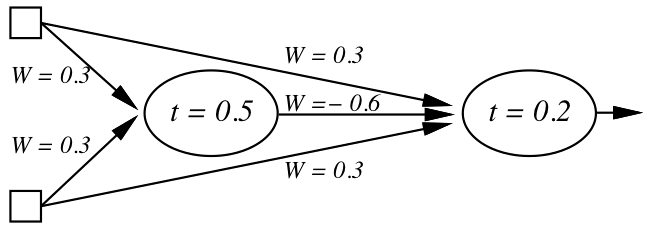
\includegraphics[width=3.5in]{./images/xor-mlp.png}
		\end{answer}

\end{enumerate} %Q1

\newpage

%Q2 30 marks
% reasoning under uncertainty
% aima chapters 13, 14, 15
\begin{figure}[h]
	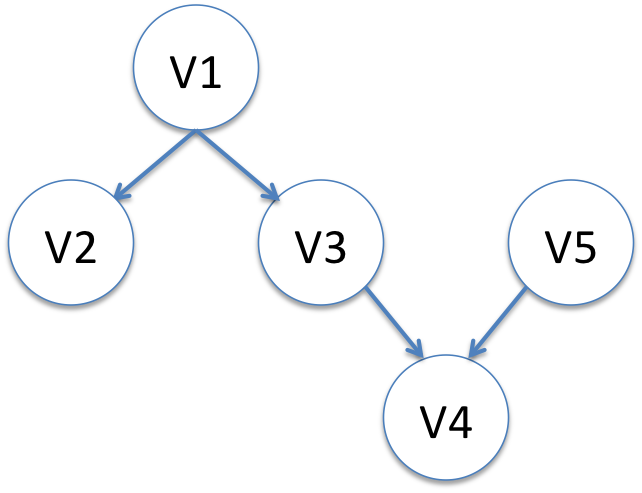
\includegraphics[width=2.5in]{./images/callan-chap5-q4.png}
	\caption{An example Bayesian network.}
	\label{fig:callan-ch5-q4}
\end{figure}

\question
\begin{enumerate}
\item Given that $P(a|b)=0.5$, $P(a)=0.3$, $P(b)=0.4$ calculate $P(b|a)$.
\marks{5}
\begin{answer}
$P(b|a)=\frac{P(a|b)\times P(b)}{P(a)}=\frac{0.5 \times 0.4}{0.3}=0.67$
\end{answer}


\item Express the joint probability distribution for the network in Figure \ref{fig:callan-ch5-q4} using the chain rule.
\marks{10}
\begin{answer}
The chain rule is: $P(x_1,\ldots,x_n) = \myprod_{i\eq 1}^n P(x_i | x_{i-1}, \dots , x_1)$.
In a properly constructed bayesian network: $\parents(X_i) \subseteq \{ x_{i-1}, \dots, x_1 \}$. 
Therefore, in a properly constructed Bayesian network: $P(x_1,\ldots,x_n) = \myprod_{i\eq 1}^n P(x_i | x_{i-1}, \dots , x_1) = \myprod_{i\eq 1}^n P(x_i|\parents(X_i))$.
So the joint probability distribution for the given network is: $P(V4|V3, V5)P(V3|V1)P(V2|V1) P(V5)P(V1)$
\end{answer}

\item  
\begin{enumerate}
\item In the context of inference in probabilistic temporal models define, in your own words. what is meant by the term \textbf{filtering}.
\marks{5}
	\begin{answer}
	Informally: filtering is the task of computing the belief state -- the posterior distribution over the current state, given all the evidence to date.
	\end{answer} 
\item Provide the equation that defines a recursive formulation of filter estimation and explain its components.
\marks{10}
	\begin{answer}
Formally: filtering involves computing the probability distribution $\pv(X_t|e_{1:t})$ where that $\X_t$ denotes the world state at time slice $t$ and $\e_{1:t}$ denotes the stream of evidence arriving from our sensors beginning at time $t=1$. This probability distribution can be recursively computed using:\\
		\begin{center}  
			\emph{$\pv(\X_{t+1}|\e_{1:t+1}) = \alpha \underbrace{\pv(\e_{t+1}|\X_{t+1})}_{Sensor~Model.}  \mysum_{x_t}  \underbrace{ \pv(\X_{t+1}|x_t)}_{Transition~Model.} \underbrace{P(x_t,|\e_{1:t})}_{Current~State~Distribution.}$}
		\end{center}
		\begin{itemize}
			\item The \textbf{current state distribution} is the probability distribution that we believe over timeslice $x_t$ given the evidence from timeslice 1 to $t$ - $\e_{1:t}$.
			\item The \textbf{transition model} describes how the world state evolves over time.
			\item The \textbf{sensor model} describes how the "sensors" -- that is evidence variables -- are affected by the actual state of the world.
		\end{itemize}
	\end{answer}
\end{enumerate}

\end{enumerate}


\newpage

%Q3
%Inductive Learning (Decision Trees)
%aima chapters 18
\question
\begin{enumerate}

\question Explain what is meant by \textbf{inductive learning}.
\marks{5}
		\begin{answer}
		Inductive Learning involves the process of learning by example � where a system tries to induce a general rule from a set of observed instances
		\end{answer}
		
	\item Suppose we generate a training set from a decision tree and then apply decision-tree learning to the training set. Is it the case that the learning algorithm will eventually return the correct tree as the training set size goes to infinity? Why or why not?
		\marks{5}
		\begin{answer}
				The algorithm may not return the''correct'' tree, but it will return a tree that is logically equivalent, assuming that the method for generating examples eventually generates all possible combinations of input attributes. This is true because any two decision tree defined on the same set of attributes that agree on all possible examples are, by de�nition, logically equivalent. The actual form of the tree may differ because there are many different ways to represent the same function. (For example, with two attributes A and B we can have one tree with $A$ at the root and another with $B$ at the root.) The root attribute of the original tree may not in fact be the one that will be chosen by the information gain heuristic when applied to the training examples. 
		\end{answer}
	
\question The following sets express the mappings between predicates $r$, $p$, $q$, $s$, $class1$ and $class2$: $r\rightarrow \{a1, a2, a5, a6 \}$, $p\rightarrow \{a2, a3, a5, a7 \}$, $q\rightarrow \{a1, a2, a6 \}$, $s\rightarrow \{(a2, f), (a1,1), (a6,f)\}$, $class1\rightarrow \{a2\}$, $class2\rightarrow \{a2, a6\}$.
\begin{enumerate}
	\item Given the above sets give a specialisation of the rule $class1(X)\leftarrow r(X) \land p(X)$ such that the rule is only satisfied by $class1$ members.
	\marks{5}
	\begin{answer}
	$class1(X)\leftarrow r(X) \land p(X) \land q(X)$
	\end{answer}
	\item Given the above sets give a rule that will correctly classify only members of $class2$.
	\marks{5}
	\begin{answer}
	$class2(X)\leftarrow s(X, f)$
	\end{answer}
\end{enumerate}

\item The FOIL inductive logic programming algorithm is considering adding a literal $l$ to a rule $r$. The extension of the rule $r$ before adding $l$ is the following set of positive and negative examples $\{+,+,+,+,+,+,-,-,-,- \}$. The extension of the rule after the literal is added (i.e. the extension of $r+l$) is $\{+,+,+,+,+,+,-,- \}$. What is the information gain of adding the literal $l$ to the rule $r$? (Note you do not need to calculate the logs in your answer ,i.e. you can express your answer as an equation containing logs).
\marks{10}
\begin{answer}

\[Foil\_Gain(L,R) \equiv t \left( \log_{2}\frac{p_{1}}{p_{1}+n_{1}} -
\log_{2}\frac{p_{0}}{p_{0}+n_{0}} \right) \]

Where
\begin{itemize}
\item $L$ is the candidate literal to add to rule $R$
\item $p_0$ = number of positive bindings of $R$
\item $n_0$ = number of negative bindings of $R$
\item $p_1$ = number of positive bindings of $R+L$
\item $n_1$ = number of negative bindings of $R+L$
\item $t$ is the number of positive bindings of $R$ also covered by $R+L$
\end{itemize}

In this instance
\begin{itemize}
\item $p_0$ = 6
\item $n_0$ = 4
\item $p_1$ = 6
\item $n_1$ = 2
\item $t$ = 6
\end{itemize}

\[Foil\_Gain(L,R) \equiv 6 \left( \log_{2}\frac{6}{6+2} -
\log_{2}\frac{6}{6+4} \right) \]

\end{answer}


\end{enumerate}
 
%Q4
%Neural Nets
\question 
\begin{enumerate}
\item Explain why  linear threshold perceptrons can represent the AND and OR functions but not the XOR function.
\marks{10}
	\begin{answer}

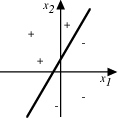
\includegraphics[width=1.5in]{./images/linear-separator.png}\\

We can think of a 2 input threshold perceptron as representing a line separator in 2D input space.In other words, the function $\sum_j W_j a_j > 0 \quad\mbox{or}\quad \vec{w} \bullet \vec{a} > 0$ defines a line in the input space and the perceptron outputs a 1 for instances lying on one side of the line and -1 for instances lying on the other side of the line.

The figure above illustrates this concept. The equation for the line in this image is $\vec{w} \bullet \vec{a} >0$. The inputs into the perceptron are $x_1$ and $x_2$; i.e. $\vec{a} = \{ x_1, x_2 \}$. 

This concept of a linear perceptron defining a line scales up into higher dimensional input space. In 3D and higher inputs space (i.e. in situations where the linear perceptron has 3 or more inputs), the linear activation function $\vec{w} \bullet \vec{a} >0$ defines a hyperplane decision surface in the $n$-dimensional space of inputs.

Data-sets of positive and negative examples that can be separated by a hyperplane are called \emph{linearly separabe}.

Of course, not all data-sets of positive and negative examples are linearly separable. The XOR function is one example of a non-linearly separable function. 

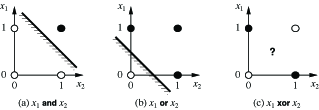
\includegraphics[width=3in]{./images/perceptron-linear.png}\\

The figure above illustrates this by comparing it with the AND and OR function which are linearly separable. In this figure black dots represent a point in the input space where the value of the function is 1, and white dots indicate a point where the value is 0.

As is evident from the images, in the AND and OR inputs spaces it is possible to draw a line that separates the black dots from the white dots. However, in the XOR space no such line exists. \emph{As a result, a threshold perceptron cannot represent the XOR function}.
	\end{answer}

\item Describe the perceptron training rule?
\marks{10}
	\begin{answer}
	Perceptrons learn by modifying the weights associated with their inputs. Consequently, the learning problem faced by perceptron training is to determine a weight vector that causes the perceptron to produce the correct $+-1$ output for each of the given training examples.

One way to learn an acceptable weight vector is to begin with random weights, then iteratively apply the perceptron to each training example, modifying the perceptron weights whenever it misclassifies an example.

Weights are modified at each step according to the \emph{perceptron training rule}, which revises the weight $w_i$ associated with input $a_i$ according to the rule:
\begin{center}
$w_i \leftarrow w_i + \Delta w_i$
\end{center}
where
\begin{center}
$\Delta w_i = \eta(t - o) a_i$
\end{center}

where t = target output, o = observed output, $\eta$ is a positive constant called the \emph{learning rate}. The role of the learning rate is to moderate the degree to which weights are changed at each step. It is usually set to some small value (e.g.$0.1$) and is sometimes made to decay as the number of weight-training iterations increases.
\end{answer}

\item Why does the perceptron learning rule converge toward successful weight values?
\marks{10}
\begin{answer}
If the training example is \emph{correctly classified} $(t-o)=0 \rightarrow \Delta w_i =0$ so \emph{no weights are updated}.

If the case of a \emph{false negative} (o=0 and t=1) we want to make the perceptron output a 1 instead of a 0 so the weights must be altered to increase the value of $\vec{w} \bullet \vec{a}$. Notice that in this case \emph{the rule will increase $w_i$} because $(t-o), \eta$ and $a_i$ are all positive.

On the other hand, in the case of a \emph{false positive} (o=1 and t=0) then \emph{the weights associated with $a_i$ will be decreased}.
\end{answer}
\end{enumerate}

%\end{enumerate}
\end{document}
